In this part, we will refer to the following : 
\begin{itemize}
	\item \emph{TP} : Number of positives predicted as such
	\item \emph{TN} : Number of negatives predicted as such
	\item \emph{FP} : Number of positives predicted as negatives
	\item \emph{FN} : Number of negatives predicted as positives
\end{itemize}
They are also illustrated in figure \ref{fig:prec_rec}.

At the end of our calculus, we generate the confusion matrix.
This matrix indicates, for any given square (i,j), how many items of the class i were predicted of class j.
An example of a confusion matrix for a binary prediction is given in figure \ref{fig:confusion}.

\begin{figure}[!h]
\centering
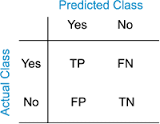
\includegraphics[width=.3\textwidth]{Images/confusion.png}
\caption{An example of a confusion matrix.}
\label{fig:confusion}
\end{figure}


In order to test the performance of our classifiers, we rely on a few indicators, processed from the confusion matrix :
\begin{itemize}
	\item \emph{Precision} indicates how many of the selected items are relevant
		\begin{equation*}
		Precision = \frac{TP}{TP+FP}
		\end{equation*}
	\item \emph{Recall} indicates how many relevant items were selected 
		\begin{equation*}
		Recall = \frac{TP}{TP+FN}
		\end{equation*}
	\item The \emph{F-Measure} takes into account both of those values
		\begin{equation*}
		F\-Measure = \frac{2\times Precision\times Recall}{Precision + Recall}
		\end{equation*}
\end{itemize}
These values are illustrated in figure \ref{fig:prec_rec}.

\begin{figure}[!h]
\centering
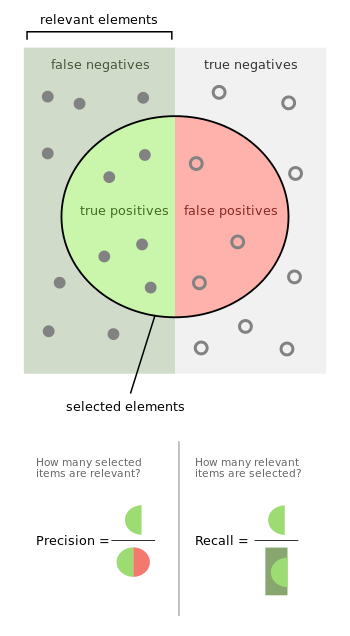
\includegraphics[width=.5\textwidth]{Images/prec_rec.png}
\caption{Precision and recall.}
\label{fig:prec_rec}
\end{figure}


For muticlass classifiers, Precision and Recall are an average of the precision and recall of the binary classifiers for each class.
\begin{equation*}
Precision_{Multiclass} = \frac{\sum_{i=0}^{n} Precision(i)}{n} 
\end{equation*}
\begin{equation*}
Recall_{Multiclass} = \frac{\sum_{i=0}^{n} Recall(i)}{n} 
\end{equation*}
